\documentclass[a4paper,12pt]{article}

% Import the deliverable package from common directory
\usepackage{../common/deliverable}

% Tell LaTeX where to find graphics files
\graphicspath{{../common/logos/}{./figures/}{../}}

\usepackage{xspace}
\usepackage{lipsum}
\usepackage[utf8x]{inputenc} % for registered and trademark symbols
\usepackage{listings}

% Set the deliverable number (without the D prefix, it's added automatically)
\setdeliverableNumber{3.3}

% Begin document
\begin{document}

% Create the title page with the title as argument
\maketitlepage{Integration of performance measuring tools}

\newpage
% Main Table using the new environment and command
\begin{deliverableTable}
    \tableEntry{Deliverable title}{Integration of Performance Measuring Tools}
    \tableEntry{Deliverable number}{D3.3}
    \tableEntry{Deliverable version}{0.1}
    \tableEntry{Date of delivery}{February 28, 2026}
    \tableEntry{Actual date of delivery}{February 28, 2026}
    \tableEntry{Nature of deliverable}{Demonstrator, pilot, prototype}
    \tableEntry{Dissemination level}{Public}
    \tableEntry{Work Package}{WP3}
    \tableEntry{Partner responsible}{BADW-LRZ}
\end{deliverableTable}

% Abstract and Keywords Section
\begin{deliverableTable}
    \tableEntry{Abstract}{\lipsum[1][1-5]}
    \tableEntry{Keywords}{performance; analysis; energy; accelerators}
\end{deliverableTable}

\newpage

\begin{documentControl}
    \addVersion{0.1}{February 10, 2026}{Ivan Pribec}{Initial draft}
%    \addVersion{0.2}{[Date]}{[Author name]}{[Description of changes]}
%    \addVersion{0.3}{[Date]}{[Author name]}{[Description of changes]}
%    \addVersion{1.0}{[Date]}{[Author name]}{Final version}
\end{documentControl}

\subsection*{{Approval Details}}
Approved by: [Name] \\
Approval Date: [Date]

\subsection*{{Distribution List}}
\begin{itemize}
    \item [] - Project Coordinators (PCs)
    \item [] - Work Package Leaders (WPLs)
    \item [] - Steering Committee (SC)
    \item [] - European Commission (EC)
\end{itemize}

\vspace*{2cm}

\disclaimer

\newpage

\tableofcontents % Automatically generated and hyperlinked Table of Contents

\newpage

\section{{Introduction}}

This deliverable provides a software framework demonstrator for the performance
analysis of large-scale simulations on EuroHPC systems including accelerators.
The intention is to provide a portable example (in terms of different hardware and software frameworks)
which is applicable to a broad range or European supercomputing,
thus supporting the transition to exascale computing.

The diversity of accelerators from multiple vendors (Nvidia, AMD, Intel) deployed
at EuroHPC centers and also national HPC sites poses a significant challenge
for scientists and engineers in terms of needed developments effort to obtain
correct, robust and performant production codes for large-scale scientific computing.

\subsection{{Purpose of the Document}}

The purpose of the demonstrator is to provide a standardized blueprint for
both library and application developers within WP1 and WP2 of the dealii.X project.
The demonstrators are also of relevance to other stakeholders in the field of finite element
software and GPU computing.

We demonstrate three distinct methodologies, presented here in descending order
of complexity and implementation effort:
\begin{itemize}
    \item Application-level profiling and manual roofline analysis
    \item Instrumentation-based approaches
    \item Sampling-based approaches
\end{itemize}

Understanding the trade-offs between these methods -- specifically regarding data
collection granularity, runtime overhead, and degree of automation -- is essential
for an information selection of the appropriate tool for a certain performance
analysis task.
Integrating these performance analysis workflows early in the software development
ccle is critical for ensuring codebases remain performant and portable across the
diverse heterogenous environments of the EuroHPC ecosystem.

\subsection{{Structure of the Document}}
\begin{itemize}
    \item Section \ref{sec:section2}: [Section Title]
    \item Section \ref{sec:section3}: [Section Title]
    \item Section \ref{sec:section4}: [Section Title]
    \item Section \ref{sec:section5}: [Section Title]
    \item Section \ref{sec:section6}: [Section Title]
\end{itemize}

\newpage

\section{{Poisson Solver Proxy App}}
\label{sec:section2}

The Bakeoff Problem (BP) based demonstrator solves the Poisson equation,
$$
\nabla^2 u = f
$$
in a 3-d box geometry, $\Omega = [0,1]^3$ discretized with hexahedral elements using
high order tensor-product polynomials.
Essential boundary conditions, $u = 0$, are applied on the domain boundar $\partial \Omega$
The degrees of freedom in the discretized system are the nodal basis values at the
Gauss-Legendre-Lobatto (GLL) knots. For a given polynomial degree $p$,
the nodal basis has $p+1$ points in each spatial dimension.

The implementation assumes deformed elements, meaning that for the
operator evaluation the metric terms (Jacobian) are used and no simplications
which could arise from aligned cartesian meshes are exploited.
This makes the proxy app more representative for scenarios with complex geometries.

Given the adjointness of the Laplace operator, and the essential boundary conditions the conjugate gradient iterative solver is used to solve the linear system.
The global system matrix is not assembled; only the operator action, i.e. the evaluation of the bilinear form is used.

The demonstrator includes both non-preconditioned and preconditioned variants
of the Poisson problem.

The non-preconditioned variant, herein nicknamed BP3.5, is designed to be close
to the CEED Bakeoff Problems. It's purpose is evaluation of the the accelerator software frameworks (Kokkos and vendor-provided frameworks), GPU kernel optimization of the bilinear form and performance analysis/estimation.

The preconditioned variant is based on the multigrid approach (CITE...).
For efficient solvers it is of critical importance to use suitable
preconditioners.
Multigrid-based preconditioners offer a very promising solution, as they are
effective at propagating information at a faster rate compared to other iterative solvers.

One of the scaling problems arising with multigrid methods is the
communication latency of the coarse-grid solver at very high MPI rank counts.

\begin{lstlisting}[caption={Script for building the BP3.5 demo}]
git clone https://github.com/dealii-X/benchmarks.git
cd benchmarks/bakeoff_problems_dealii

# checkout specific commit (git checkout <commit_hash>)

cmake -B build -S src \
    -DCMAKE_CXX_COMPILER="$(which mpicxx)" \
    -DDEAL_II_DIR=<dealii_installation_path>
cmake --build build
\end{lstlisting}

\begin{lstlisting}[caption={Script for building the BK benchmarks}]
git clone https://github.com/dealii-X/benchmarks.git
cd benchmarks/sum_factorization
cmake -B build -S . \
    -DCMAKE_CXX_COMPILER="$(which cxx)" \
    -DKokkos_DIR=<Kokkos_installation_path>
cmake --build build -j <jobs>
\end{lstlisting}

\subsection{{BP3.5 Problem}}

The Bakeoff Problem 3 (BP3) acts as a proxy-app solving a Poisson equation,
a common step in fluid mechanics and/or scalar transport models, both of which are highly relevant also to biological systems such as organs.

While the geometry is a simple cube ("a brick"), we emphasize that all our
tests have been performed using general irregular data structures, such that
we do not expect significant deviations in the case of more general hexahedral grids.

It is worth highlighting that the problem setup is very similar to the HPCG benchmark.
The main differences are the choice of numerical discretization method, namely finite differences for HPCG and finite elements for BP.
HPCG is primilary a hardware benchmark; the accuracy of the finite difference stencil is set in advance. The throughput in terms of floating points operations is measured for a fixed time or a fixed number of steps. Due to the memory intensive storage of
the matrix, the HPCG problem is typically limited by the memory bandwidth.

Other differences are the BP problems do not include any preconditioner.

TODO: check if HPCG uses preconditioners.

The Poisson solver step is often formulated implicitly, requiring the solution
of a large system of linear equations.

The proxy problem is a hybrid of the two problems BP3 and BP5, since
it uses a different number of quadrature points.
(Is this over-integration, or is it still exact?)

\subsection{{Bakeoff Kernels}}

In our experiments, the AMD MI210 has shown good performance of BK1 and BK5 kernels, particularly in the situations where the wavefront size perfectly matches the
number of quadrature points.

\cite{Karp2023} observed that the use of 1-d thread blocks enabled higher performance on the AMD Instinct MI250X GPU, compared to launching 2-d or 3-d thread blocks per element, despite the latter mapping naturally to the tensor product kernels.
This stood in contrast to Nvidia GPUs where 2-d/3-d thread blocks were used.



ce difference between the use of 1-d and 2-d thread blocks when
indexing elements. In contrast to Nvidia GPUs, where the use of 2-d and 3-d thread blocks

 one-dimensional thread indexing provided better performance than  multi-dimensional on the AMD MI250X devices in LUMI, however the cause remained uncertain.

We speculate that optimization of thread-block sizes and or the introduction of padding to prevent bank conflicts, could yield further improvements and will be the subject of future work.

\begin{figure}
\centering
%
\includegraphics[width=0.8\textwidth]{BK1_1}
\caption{BK1 performance results on Nvidia GH200 GPU with Kokkos programming model.}
\label{fig:BK1_GH200}
\end{figure}

\begin{figure}
\centering
%
\includegraphics[width=0.8\textwidth]{BK1_1}
\caption{BK1 performance results on Intel Data Center GPU Max 1550 (``Ponte Vecchio'') with Kokkos programming model.}
\label{fig:BK1_PVC}
\end{figure}

\begin{figure}
\centering
%
\includegraphics[width=0.8\textwidth]{BK1_1}
\caption{BK1 performance results on AMD Instinct MI210 with Kokkos programming model.}
\label{fig:BK1_AMD}
\end{figure}

\newpage
\section{{Performance Analysis Tools}}
\label{sec:section3}

The complexity of both the the software in question and the target hardware,
limit what can be inferred solely using application-based performance reporting.

Luckily, a growing amount of both vendor-provided and open-source software can provide the in-depth analysis capabalities, based on hardware performance counters, micro-benchmarking, and automatic analysis capabilities which can make performance optimization easier.

\subsection{{Nvidia NSight Systems}}
\begin{itemize}[left=1em, itemsep=0pt, topsep=0pt] 
    \item \lipsum[10][1-2]
    \item \lipsum[10][3-4]
    \item \lipsum[10][5-6]
\end{itemize}

NSight Systems provides a system-wide timeline view, showing how the CPU and GPU
executions. It also provides statistics about API calls, overhead and memory transfers
(HtoD/DtoH).

To create a profile, we launch the application with the command\footnote{We use \texttt{<>} to denote mandatory arguments, and \texttt{[]} to denote optional arguments}
\begin{verbatim}
> nsys profile <target> [target-options]
\end{verbatim}
Further command switch options can be provided to control what is collected.

It is useful to collect profiling tool invocations either in the project readme file or scripts for future reference.

\subsection{{Intel® VTune™ Profiler VTune™}}

The VTune Profiler\footnote{\url{https://www.intel.com/content/www/us/en/developer/tools/oneapi/vtune-profiler.html}} ...


\subsubsection{Intel Application Performance Snapshot}

The Intel Application Performance Snapshot is a helpful tool for Linux OS which provides a quick
overview of compute intensive applications running on x86-64 architecture.

\begin{verbatim}
> aps --result-dir=<foldername> <target> [target-options]
\end{verbatim}

\subsubsection{VTune Profiler}

\begin{verbatim}
> vtune -quiet -collect gpu-offload -r vtune_gpu_offload <executable>
> vtune -quiet -collect gpu-hotspots -r vtune_gpu_hotspots ...
\end{verbatim}


Cheat sheet\footnote{\url{https://www.intel.com/content/dam/develop/external/us/en/documents/vtune-profiler-cheat-sheet.pdf}}

\subsection{Intel® Advisor}

The tool also support a command-line interface (CLI), useful to collect results
on remote systems and/or under batch-scheduling constraints.

Collection of the roofline data is performed using the command
\begin{verbatim}
> advisor --collect=roofline --profile-gpu -- <executable>
\end{verbatim}
To obtain line profiling data linked to the source file, the executable must be (re)compiled with the following \texttt{icpx} options: \texttt{-fdebug-info-for-profiling -gline-tables-only}.

\begin{figure}
\centering
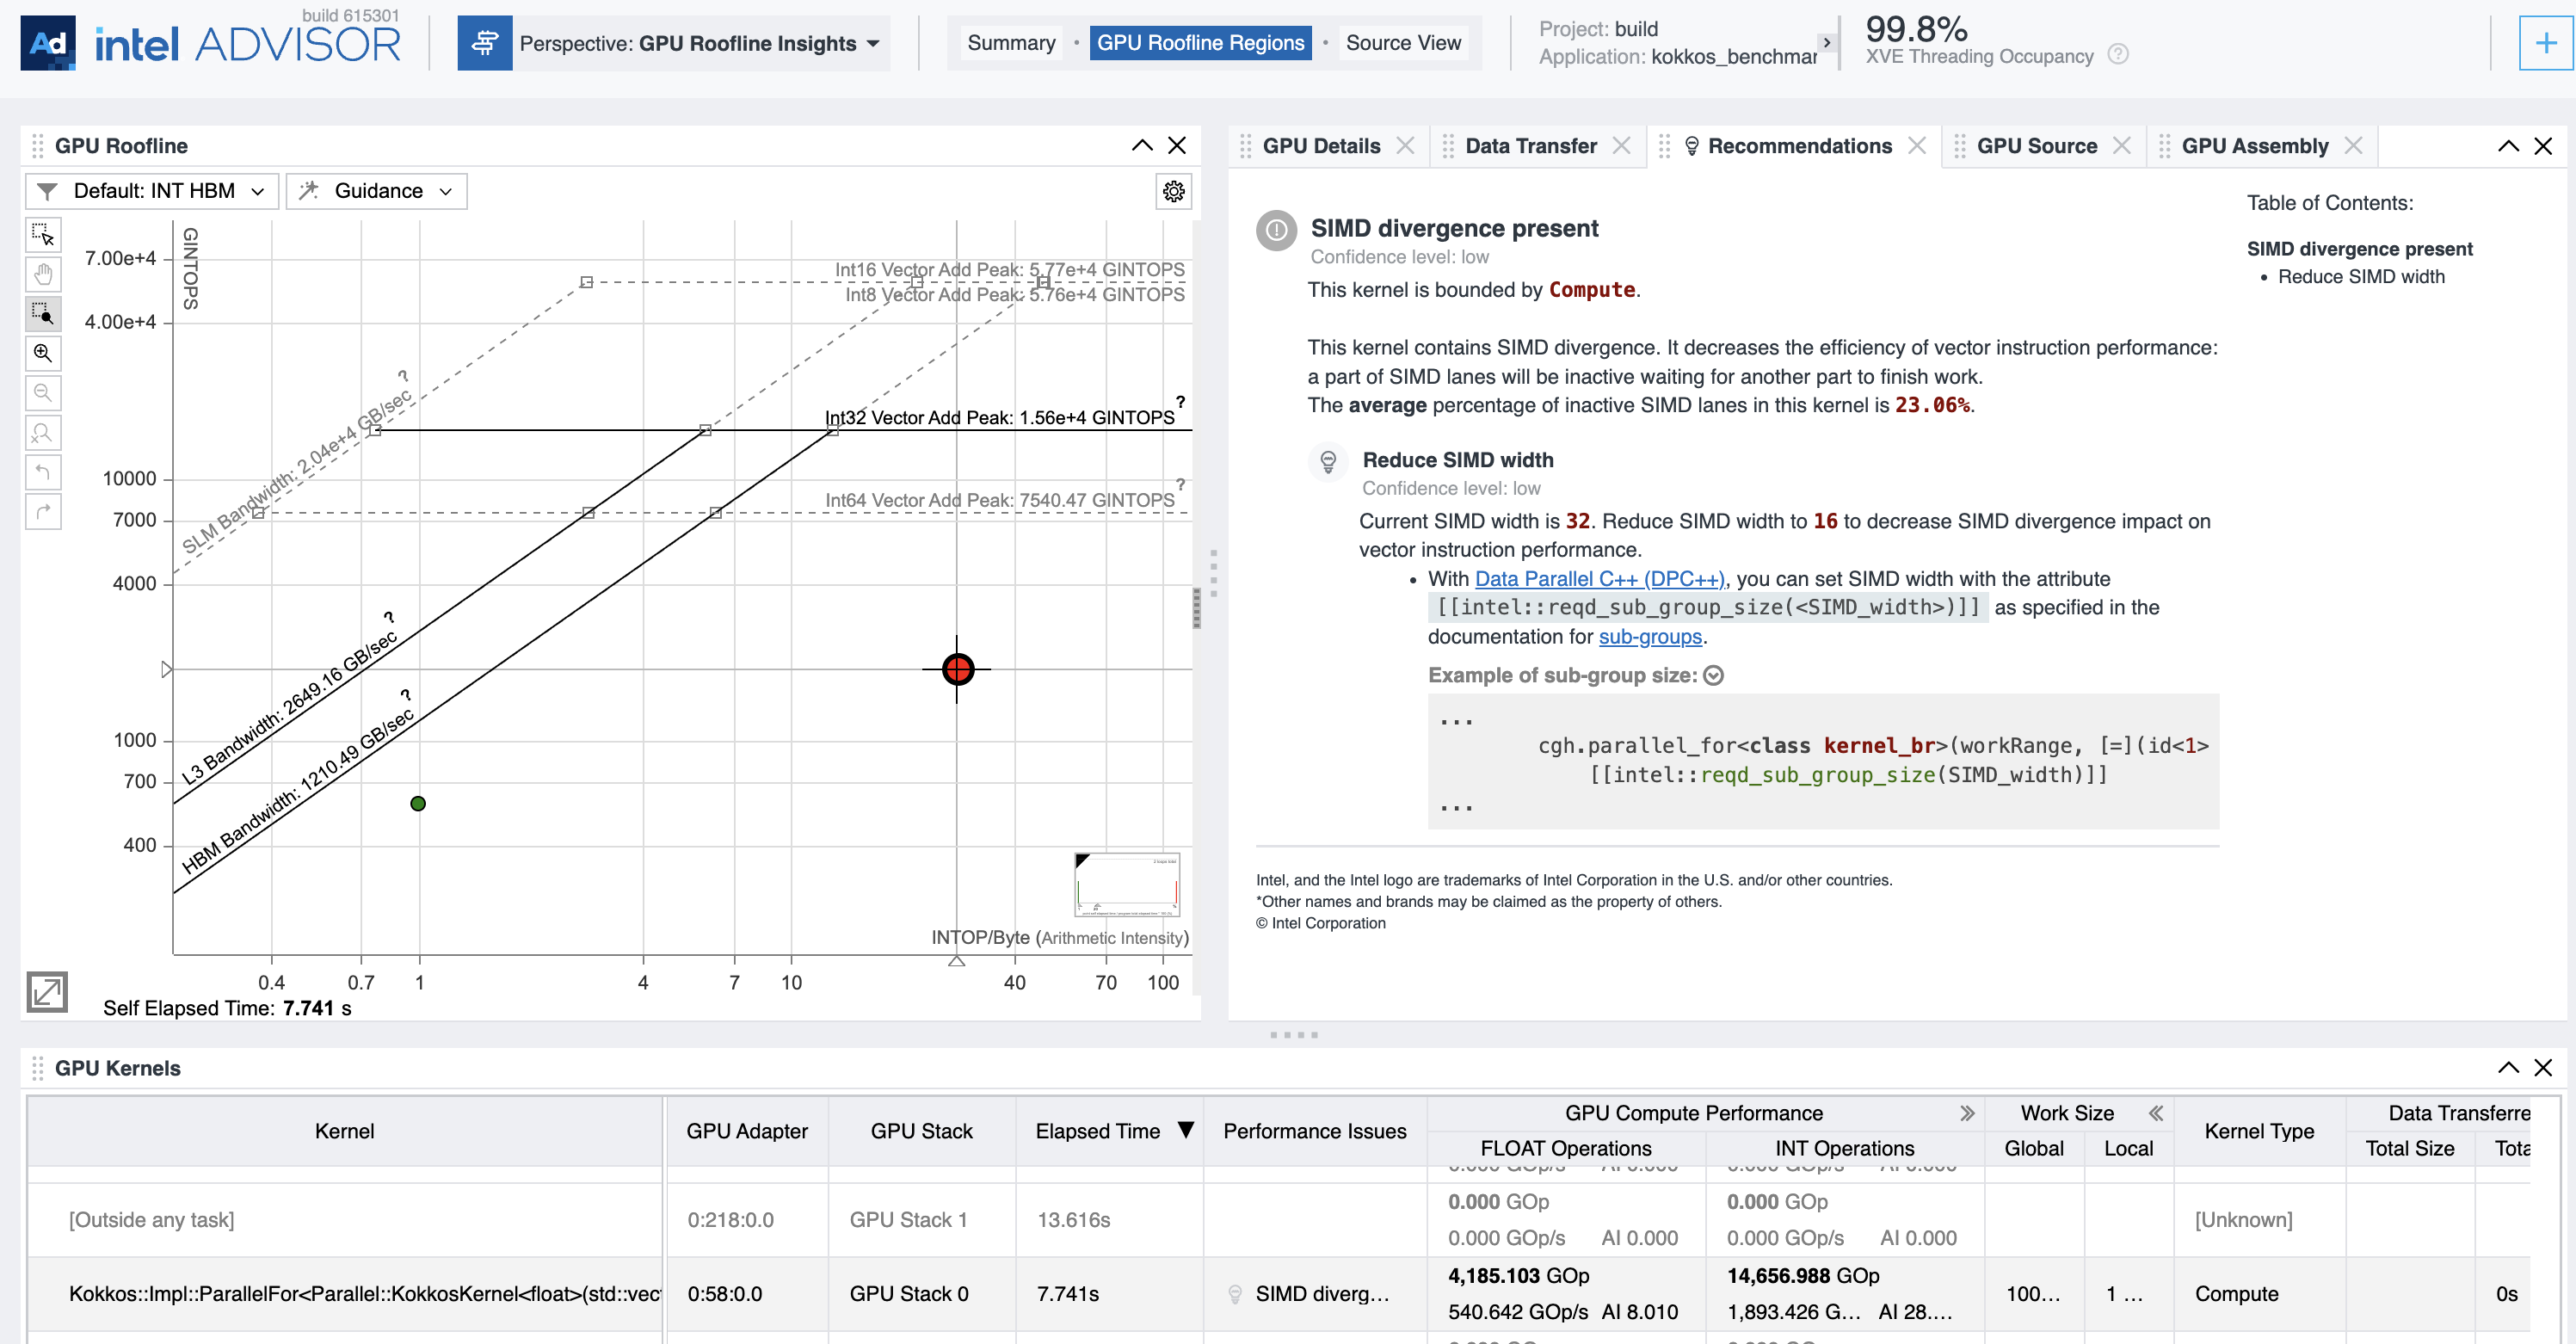
\includegraphics[width=0.95\textwidth]{advisor-screenshot-2025-07-24}
\caption{Exemplary view of Bakeoff Kernel result in Intel Advisor.}
\label{fig:intel_advisor}
\end{figure}


\subsection{LIKWID}

The LIKWID Performance Tools\footnote{\url{https://hpc.fau.de/research/tools/likwid/}}
developed by Erlangen National High Performance Computing Center (NHR@FAU) are a suite
of command-line applications for performance monitoring and benchmarking.
It supports Intel, AMD, and ARM CPU architectures on GNU/Linux operation system.
Recent versions of the tools have also added support for Nvidia and AMD GPUs.

For  the LIKWID Marker API is used. In this approach
regions of interest in the code are tagged/registered for performance counter collection.

Use of the Marker API enables measuring named regions of the code.

\begin{lstlisting}[caption={Minimal example of using LIKWID Marker API for CPU instrumentation}]
#include <likwid-marker.h>
int main() {
  LIKWID_MARKER_INIT;
  LIKWID_MARKER_THREADINIT;
  LIKWID_MARKER_START("matvec");
  /* region of interest we measure */
  LIKWID_MARKER_STOP("kernel");
  LIKWID_MARKER_CLOSE;
  return 0;
}
\end{lstlisting}
In practice, the Marker API calls are often controlled using preprocessor conditional text inclusion:
\begin{verbatim}
#ifdef LIKWID_PERFMON
/* LIKWID header or Marker API calls*/
#endif
\end{verbatim}
to allow selection of the instrumented code at compilation time using
the definition \texttt{-D LIKWID_PERFMON}.

After building the instrumented executable it is invoked with the Likwid performance counter wrapper:
\begin{verbatim}
> likwid-perfctr [options] <executable>
\end{verbatim}

The listing below shows an example of the expected output using the metric group:
\begin{lstlisting}[caption={Output of \texttt{likwid-perfctr} for the serial BK1 benchmark (CPU-only).}]
...
\end{lstlisting}
Likwid supports several pre-existing metric groups to enable.


\newpage
\section{{Energy Measurement}}
\label{sec:section4}

The assesment of energy usage is an often-overlooked aspect in computing.
While the energy costs are often ignored for software running on personal/desktop computers, the large scale of modern HPC systems incurs significant runtime
costs for electricity.

The performance per Watt has been increasing steadly in the last decades, driven
by improvements in hardware architecture and design.
Nonetheless, software factors also have a very large influence.
A famous place where this plays out is the memory access pattern on modern GPUs,
where the use of coalesced loading patterns greatly improves both performance
and the expended enegy (CITE Steven Jones talk).

The plethora of factors influencing energy usage, including frequency,
software intensity, memory access patterns and parallelism, make reproducible measurement of energy challenging for the final scientific users.


\begin{center}
    \begin{table}[h!]
    \small
    \caption{[Table Caption]}
    \renewcommand{\arraystretch}{1.25}
    \label{tab:example_table}
    \begin{tabular}{|l|l|l|c|}
    \hline
    \textbf{Column 1} & \textbf{Column 2} & \textbf{Column 3} & \textbf{Column 4} \\
    \hline
    Item 1 & Description & Category & Value \\
    Item 2 & Description & Category & Value \\
    Item 3 & Description & Category & Value \\
    \hline
    \end{tabular}
    \end{table}
\end{center}

\newpage

\section{{[Section Title]}}
\label{sec:section5}

\lipsum[14-15]

\subsection{{[Subsection Title]}}
\lipsum[16]

\subsection{{[Subsection Title]}}
\begin{itemize}[left=1em, itemsep=0pt, topsep=0pt] 
    \item \textbf{[Item Title]}: \lipsum[17][1-2]
    \item \textbf{[Item Title]}: \lipsum[17][3-4]
    \item \textbf{[Item Title]}: \lipsum[17][5-6]
\end{itemize}

\newpage

\section{{[Section Title]}}
\label{sec:section6}

\lipsum[18-19]

\begin{center}
\resizebox{\textwidth}{!}{
\begin{tabular}{|l|l|l|}
\hline
\textbf{Column 1} & \textbf{Column 2} & \textbf{Column 3} \\
\hline
Item 1 & Description & Value \\
\hline
Item 2 & Description & Value \\
\hline
Item 3 & Description & Value \\
\hline
\end{tabular}}
\label{tab:example_table2}
\end{center}

\newpage 

\section{{Conclusion}} \label{sec:conclusion}

\lipsum[20]



\bibliographystyle{plainnat}
% refs.bib in the same folder
\bibliography{refs}

\label{MyLastPage}

\end{document}
